%Exemplo de capitulo

\chapter{Introdução}

\begin{figure}[!htb]
	\centering
	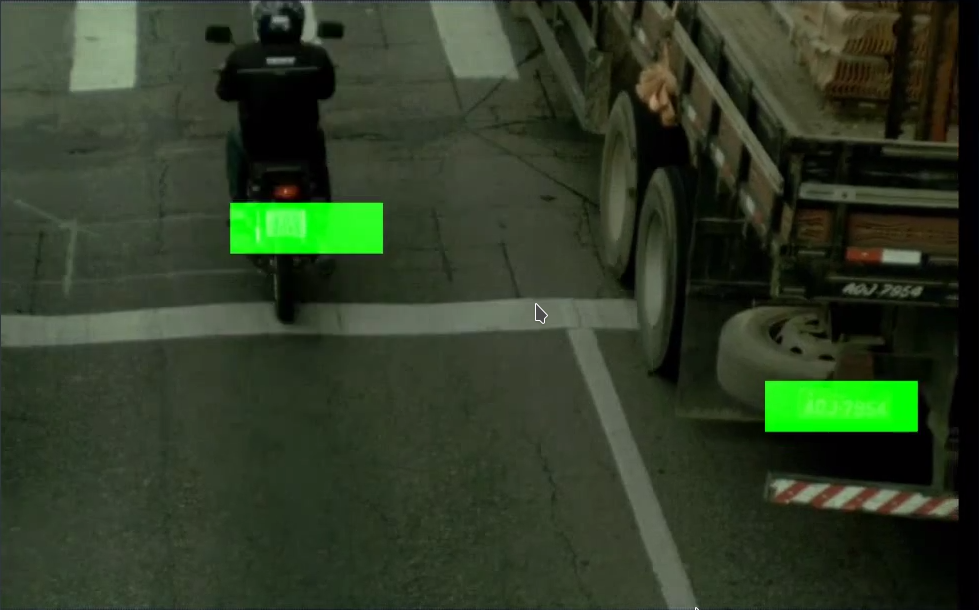
\includegraphics[scale=0.5]{cap1_resultado_esperado.png}
	\caption{Resultado esperado}
	\label{fig:cap1_resultado_esperado}
	(próprio autor).
\end{figure}

Soluções de monitoração e fiscalização de veículos apresentam
uma grande demanda por sistemas de visão computacional. Seja
para contar tráfego, fiscalizar o uso das vias, monitorar
rodízios ou para cobrar pedágios, a capacidade de obter
informações a partir de imagens é de grande interesse, sendo parte integrante
de uma solução típica \cite{anagnostopoulos2008license}.  Existem
soluções propostas para parte destes problemas, no entanto há a
possibilidade da busca por estratégias com menor custo ou melhor
desempenho, à medida que avanços no campo do reconhecimento de
imagens acontecem.

Redes neurais convolucionais (\sigla{CNN}{\emph{Convolutional neural network},
rede neural convolucional}, convolutional neural networks)
são tipos de redes neurais biologicamente inspiradas no conceito
de campos receptivos \cite{hubel1968receptive}. Este tipo de
rede neural pode ser alimentado
diretamente com os \emph{pixels} da imagem \cite{lecun1998gradient}. O
advento das Redes Neurais Convolucionais Profundas (\sigla{DCNN}{\emph{Deep
convolutional neural network}, rede neural convolucional profunda}, deep CNN)
viabilizou um grande salto no desempenho de classificação para alguns casos.
O uso de mais camadas permite níveis maiores de
abstração na análise da imagem, o que resulta em maior taxa de
acerto, ao custo de maior tempo de treinamento. Este tipo de rede
neural representa o atual estado-da-arte em reconhecimento de
imagens \cite{szegedy2015going}.

\section{Objetivo}
O objetivo deste trabalho é desenvolver uma abordagem para
treinamento e uso de redes neurais convolucionais para para a
construção de um sistema robusto e eficiente de localização de
placas de veículos em vídeo, e realizar uma implementação para
medição de dados de desempenho. A figura \ref{fig:cap1_resultado_esperado}
mostra um exemplo de saída que se pretende obter.

\section{Estrutura da Monografia}
O restante deste trabalho é organizado da seguinte forma: O
capítulo 2 discorre sobre redes neurais convolucionais em geral,
comparando-as com as redes neurais não-convolucionais. Como este
tópico é relativamente novo optou-se por fazer sua apresentação
o mais cedo possível no documento. O capítulo 3 é uma revisão da
bibliografia atual sobre detecção e localização de placas veiculares. O
capítulo 4 apresenta uma proposta de um método para aplicar redes neurais
convolucionais para localizar placas veiculares. O capítulo 5 apresenta uma
implementação do método proposto, experimentos e os seus resultados. O
capítulo 6 apresenta as conclusões deste trabalho.

